\documentclass[12pt,a4paper]{article}

% ─── Encodage et langue ───────────────────────────────────────────────────────
\usepackage[utf8]{inputenc}
\usepackage[T1]{fontenc}
\usepackage[french]{babel}

% ─── Mise en page ─────────────────────────────────────────────────────────────
\usepackage[top=2.5cm,bottom=2.5cm,left=2.5cm,right=2.5cm]{geometry}
\usepackage{parskip}
\setlength{\parindent}{0pt}

% ─── Typographie ──────────────────────────────────────────────────────────────
\usepackage{lmodern}
\usepackage{microtype}

% ─── Couleurs et boîtes ───────────────────────────────────────────────────────
\usepackage{xcolor}
\usepackage{tcolorbox}
\tcbuselibrary{skins,breakable}

\definecolor{bertblue}{RGB}{37,99,235}
\definecolor{bertlightblue}{RGB}{219,234,254}
\definecolor{warnorange}{RGB}{234,88,12}
\definecolor{warnlight}{RGB}{255,237,213}
\definecolor{tipgreen}{RGB}{22,163,74}
\definecolor{tiplight}{RGB}{220,252,231}
\definecolor{sectiongray}{RGB}{248,250,252}
\definecolor{ruleblue}{RGB}{59,130,246}

% ─── Boîtes d'information ─────────────────────────────────────────────────────
\newtcolorbox{note}[1][]{
  colback=bertlightblue,colframe=bertblue,fonttitle=\bfseries,
  title={#1},breakable,arc=3pt,boxrule=0.8pt
}
\newtcolorbox{warnbox}[1][Attention]{
  colback=warnlight,colframe=warnorange,fonttitle=\bfseries,
  title={#1},breakable,arc=3pt,boxrule=0.8pt
}
\newtcolorbox{tipbox}[1][Astuce]{
  colback=tiplight,colframe=tipgreen,fonttitle=\bfseries,
  title={#1},breakable,arc=3pt,boxrule=0.8pt
}
\newtcolorbox{critbox}[1][Problème critique]{
  colback=warnlight,colframe=red!70!black,fonttitle=\bfseries,
  title={#1},breakable,arc=3pt,boxrule=0.8pt
}

% ─── Tableaux ─────────────────────────────────────────────────────────────────
\usepackage{booktabs}
\usepackage{tabularx}
\usepackage{array}
\usepackage{multirow}
\newcolumntype{L}[1]{>{\raggedright\arraybackslash}p{#1}}
\newcolumntype{C}[1]{>{\centering\arraybackslash}p{#1}}
\setlength{\tabcolsep}{10pt}
\renewcommand{\arraystretch}{1.5}
\usepackage{tablefootnote}

% ─── Mathématiques ────────────────────────────────────────────────────────────
\usepackage{amsmath,amssymb}

% ── Graphics ───────────────────────────────────────────────────────────────────
\usepackage{graphicx}
\graphicspath{{img/}{../img/}{../../img/}{../../../img/}{../../../../img/}}

% ── Schémas ───────────────────────────────────────────────────────────────────
\usepackage{tikz}
\usetikzlibrary{calc}
\usetikzlibrary{arrows.meta, positioning, shapes.geometric, fit}

% ── wrapfigure ─────────────────────────────────────────────────────────────────
\usepackage{wrapfig}
\usepackage{float}

% ─── Code ─────────────────────────────────────────────────────────────────────
\usepackage{listings}
\lstset{
  basicstyle=\ttfamily\small,
  backgroundcolor=\color{sectiongray},
  frame=single,framerule=0.4pt,rulecolor=\color{gray!60},
  breaklines=true,
  keywordstyle=\color{bertblue}\bfseries,
  commentstyle=\color{gray},
  stringstyle=\color{tipgreen},
  showstringspaces=false,
  xleftmargin=8pt,xrightmargin=8pt,
  aboveskip=6pt,belowskip=6pt
}

\usepackage{algorithm}
\usepackage{algpseudocode}

% ─── En-têtes et pieds de page ────────────────────────────────────────────────
\usepackage{fancyhdr}
\pagestyle{fancy}
\fancyhf{}
\lhead{\small Compte-rendu technique — Étape 2 EXTRA}
\rhead{\small LARROUX Logan}
\cfoot{\thepage}
\renewcommand{\headrulewidth}{0.4pt}

% ─── Titres de sections ───────────────────────────────────────────────────────
\usepackage{titlesec}
\titleformat{\section}{\large\bfseries}{}{0pt}{}[\titlerule]
\titleformat{\subsection}{\normalsize\bfseries}{}{0pt}{}
\titleformat{\subsubsection}{\normalsize\itshape}{}{0pt}{}

% ─── Liens ────────────────────────────────────────────────────────────────────
\usepackage{hyperref}
\hypersetup{colorlinks=true,linkcolor=bertblue,urlcolor=bertblue}

% ─── Divers ───────────────────────────────────────────────────────────────────
\usepackage{enumitem}
\usepackage{graphicx}

% ══════════════════════════════════════════════════════════════════════════════
\begin{document}

% ─── Page de garde ────────────────────────────────────────────────────────────
\begin{titlepage}
  \centering

  \vspace{3cm}

  {\fontsize{20}{22}\selectfont\bfseries
    COMPTE-RENDU TECHNIQUE\\
    Analyse de conversations patient-thérapeute\\
    sur la santé mentale\par}
  {\color{blue!70!black}\rule{0.5\textwidth}{1.5pt}\par}
  \vspace{0.5cm}

  {\large\bfseries Auteur: LARROUX Logan \\
                  Encadrante : Lynda Tamine-Lechani\par}

  {\normalsize\itshape
    Équipe :\\[0.3em]
    Ulysse Chasseigne, Idir Yahiaoui, Bantsoukissa Laure,\\
    Cruz Fernandes Diogo, Emin Belkheir, Esso-Y-N Trésor PANA,\\
    Logan Larroux, Yvan Sellier, Victor Blanquart--Blanchet, Lucas Da Silva\par}

  \vspace{0.8cm}
  {\fontsize{14}{18}\selectfont\today\par}

  \vspace{1cm}
  \begin{tabular}[t]{c}
    \centering
    
\includegraphics[height=1.5cm]{universite-de-toulouse-logo.png}
    \hspace{10px}
    {
\includegraphics[height=1.5cm]{IRIT_logo.png}}
    \hspace{10px}
    \raisebox{0.70cm}{\normalsize [Info5.BE-SHS]\par}
  \end{tabular}

  \vfill

  {\color{blue!70!black}\rule{\textwidth}{0.4pt}\par}
  \vspace{0.4cm}
  {\small Données : \href{https://www.kaggle.com/datasets/thedevastator/nlp-mental-health-conversations}{Kaggle --- NLP Mental Health Conversations}\par
                    \href{https://www.kaggle.com/datasets/suchintikasarkar/sentiment-analysis-for-mental-health}{Kaggle --- Sentiment Analysis for Mental Health}\par}
  \vspace{0.2cm}
  {\small Code : \href{https://github.com/cypnet/Analyse-de-conversations-sur-la-sant-mentale}{GitHub --- branche main}\par}
  \vspace{0.5cm}
\end{titlepage}

% ─── Table des matières ───────────────────────────────────────────────────────
\tableofcontents
\newpage

% ══════════════════════════════════════════════════════════════════════════════
\section{Contexte, objectifs et organisation}

Ce document est un complément à l'étape~2 du projet. Tandis que la partie principale de
l'étape~2 portait sur des méthodes classiques de classification (Naive Bayes, Régression
Logistique, LinearSVC en supervisé~; K-Means en non supervisé), ce notebook extra
introduit une approche radicalement différente reposant sur \textbf{BERT} (\textit{Bidirectional
Encoder Representations from Transformers}).

\textbf{L'objectif reste identique~:} produire un classificateur de sentiments sur des textes liés à la
santé mentale, en s'appuyant sur le même corpus d'entraînement
(\texttt{Combined\_Data.csv} — \textit{Sentiment Analysis for Mental Health, Kaggle \footnote{lien du dataset: \href{https://www.kaggle.com/datasets/suchintikasarkar/sentiment-analysis-for-mental-health}{https://www.kaggle.com/datasets/suchintikasarkar/sentiment-analysis-for-mental-health}}}).\\
Ce qui change, c'est \textbf{la profondeur de la représentation~:} là où TF-IDF ne comptait que des
mots, BERT modélise le langage dans toute sa complexité contextuelle.

\textbf{Trois variantes de BERT} sont implémentées, dont l'une d'entre elles grandement privilégié par l'équipe. 
Elles sont ensuite comparées entre elles et avec les résultats du notebook principal~:

\begin{center}
\begin{tabular}{@{}llL{4cm}L{3cm}@{}}
  \toprule
  Modèle & Nom court & Description & Membres \\
  \midrule
  A & BERT sans fine-tuning & Extraction de features, poids gelés & Diogo \\
  B & BERT avec fine-tuning & Tous les poids mis à jour sur notre dataset & Diogo, Ulysse, Emin, Victor \\
  C & BERT spécialisé + fine-tuning & Modèle pré-entraîné sur des sentiments (\textit{Hugging Face}) puis fine-tuné & Logan \\
  \bottomrule
\end{tabular}
\end{center}

\begin{note}[Remarque]
Les métriques d'évaluation utilisées sont identiques à celles de l'étape~2 (accuracy,
classification report, matrice de confusion) afin de permettre une comparaison directe.
\end{note}

\pagebreak
% ══════════════════════════════════════════════════════════════════════════════
\section{Qu'est-ce que BERT~?}

\subsection{Définition générale}

BERT (\textit{Bidirectional Encoder Representations from Transformers}) est un modèle
de langage développé par Google en 2018. Il repose sur
l'architecture \textbf{Transformer}, mais n'en utilise que la partie \textbf{encodeur}.

Concrètement, un encodeur transforme une séquence de tokens en une
séquence de vecteurs denses appelés \textbf{représentations contextuelles}~: chaque token
se voit attribuer un vecteur dont le contenu dépend de l'ensemble de la phrase (et non du
seul mot considéré). Ce mécanisme repose sur la \textbf{self-attention multi-têtes}, qui
permet à chaque token de "regarder" tous les autres tokens simultanément et de pondérer
leur importance. 

BERT empile ainsi 12 couches (version \textit{base}) ou 24 couches
(version \textit{large}) de ce bloc encodeur, ce qui lui permet de construire des
représentations de plus en plus abstraites et nuancées au fil des couches. Le décodeur
(utilisé pour générer du texte, comme dans GPT) est délibérément absent~: BERT produit
une \textbf{compréhension} du texte, pas une génération.

De plus, sa particularité fondamentale est d'être \textbf{bidirectionnel}~: contrairement aux
modèles précédents qui lisaient le texte uniquement de gauche à droite (ou de droite à
gauche), BERT lit le contexte dans les deux directions simultanément.

\vspace{10mm}

\begin{note}[Exemple d'ambiguïté résolue par la bidirectionnalité]
« Le chat mange la souris »\\[4pt]
BERT comprend le mot \textit{mange} en regardant à la fois \textit{chat} (contexte gauche)
et \textit{souris} (contexte droit) en une seule passe — ce qu'un modèle unidirectionnel
ne peut pas faire.
\end{note}

\pagebreak

\subsection{Étapes d'apprentissage}

L'apprentissage de BERT se déroule en deux phases distinctes.

\subsubsection{1. Pré-entraînement (non supervisé)}

Avant toute tâche spécifique, BERT est pré-entraîné sur d'énormes corpus (Wikipedia
anglophone, BooksCorpus, etc.) via deux tâches auto-supervisées~:

\begin{itemize}[leftmargin=1.5cm]
  \item \textbf{Masked Language Model (MLM)~:} environ 15\,\% des tokens sont masqués
    aléatoirement et le modèle doit les prédire à partir du contexte.
    Exemple~: \texttt{« Le [MASK] mange la souris »} $\rightarrow$ prédit \texttt{chat}.
  \item \textbf{Next Sentence Prediction (NSP)~:} le modèle apprend à déterminer si
    deux phrases se suivent logiquement dans un texte ou sont juxtaposées aléatoirement.
\end{itemize}

\textbf{Cette phase est entièrement non supervisée}~: aucune annotation humaine n'est requise.
Elle permet à BERT d'acquérir une compréhension riche et générale du langage.

\subsubsection{2. Fine-tuning supervisé}

C'est ici qu'intervient l'apprentissage \textbf{supervisé}. On reprend le BERT pré-entraîné
et on l'adapte à une tâche précise avec des données étiquetées, en ajoutant une petite
couche de sortie~:

\begin{center}
\begin{tabular}{@{}L{6cm}L{4.5cm}L{5cm}@{}}
  \toprule
  Tâche & Exemple & Couche ajoutée \\
  \midrule
  Classification de texte & Sentiment positif/négatif & Dense sur le token \texttt{[CLS]} \\
  NER\footnotemark & Identifier noms, lieux\ldots & Dense sur chaque token \\
  Question-Réponse & Extraire une réponse d'un passage & Deux classifieurs (début/fin) \\
  Similarité de phrases & Phrases équivalentes~? & Dense sur \texttt{[CLS]} \\
  \bottomrule
\end{tabular}
\end{center}
\footnotetext{Named Entity Recognition ou reconnaissance d'entités nommées en français}

Le fine-tuning ne nécessite que peu de données étiquetées et peu d'epochs, car BERT
a déjà appris une représentation riche du langage lors du pré-entraînement.

\subsubsection{Tokenisation spécifique~: WordPiece}

BERT utilise un \textbf{tokeniseur WordPiece}~: les mots rares ou inconnus sont découpés
en sous-mots, ce qui garantit que tout vocabulaire peut être représenté.

\begin{lstlisting}[language={}]
"unhappiness"  ->  ["un", "##happi", "##ness"]
\end{lstlisting}

Deux tokens spéciaux sont systématiquement ajoutés~:
\begin{itemize}[leftmargin=1.5cm]
  \item \texttt{[CLS]} en début de séquence~: sa représentation finale encode
    l'information globale de la phrase et sert d'entrée à la tête de classification.
  \item \texttt{[SEP]} pour séparer deux segments distincts.
\end{itemize}

\vspace{10mm}
\begin{figure}[H]
\begin{center}
\begin{tikzpicture}[
  scale=0.85,
  transform shape,
  node distance=8mm,
  >=Latex,
  box/.style={rounded corners, draw=blue!70!black, thick, fill=blue!5, align=center, text width=4cm, minimum height=1.2cm, inner sep=6pt, font=\small},
  method/.style={box, font=\footnotesize, text width=2cm, minimum height=0.8cm, node distance=4mm},
  group/.style={draw=red!75!black, rounded corners, dashed, inner sep=12pt, thick},
  subgroup/.style={group, draw=green!70!black, inner sep=8pt},
  arrow/.style={-Latex, thick, draw=blue!70!black},
  line/.style={thick, draw=blue!70!black}
]

\node[box] (text) {Texte brut\\
"Le chat mange la souris"};

\node[box, right=of text, text width=5cm] (token) {Tokenisation\\ \texttt{[CLS] Le chat mange la souris [SEP]}};

\node[box, right=of token] (embed) {Embeddings\\
Token + Position + Segment};

\node[box, below=of embed, fill=green!10, text width=5cm] (bert) {BERT Encoder\\
Multi-head Self-Attention\\
12 couches Transformer};

\node[box, left=of bert] (cls) {Vecteur [CLS]};

\node[box, left=of cls] (dense) {Dense Layer + Softmax};

\node[box, below=of dense, fill=red!10] (output) {Classe prédite\\
Positif};

\draw[arrow] (text) -- (token);
\draw[arrow] (token) -- (embed);
\draw[arrow] (embed) -- (bert);
\draw[arrow] (bert) -- (cls);
\draw[arrow] (cls) -- (dense);
\draw[arrow] (dense) -- (output);

\end{tikzpicture}
\caption{\centering\small Schéma simplifié du pipeline de BERT pour la classification de texte.}
\end{center}
\end{figure}

\pagebreak

\subsection{Points forts de BERT}

\begin{itemize}[leftmargin=1.5cm]
  \item \textbf{Représentations contextuelles~:} le même mot reçoit des vecteurs
    différents selon son contexte — \textit{banque} n'est pas la même chose dans
    « banque financière » et « banque de sable ».
  \item \textbf{Transfert de connaissances efficace~:} un BERT pré-entraîné une seule
    fois peut être fine-tuné pour des dizaines de tâches différentes avec peu de données.
  \item \textbf{Écosystème riche~:} des variantes existent pour de nombreux besoins:
  \begin{itemize}[leftmargin=1.5cm]
    \item \textbf{RoBERTa} (plus robuste), 
    \item \textbf{CamemBERT} (français),
    \item \textbf{DistilBERT} (plus léger et rapide), 
    \item etc. 
  \end{itemize}
\end{itemize}

\subsection{Limites de BERT}

\subsubsection{Coût computationnel élevé}

C'est probablement la limitation la plus concrète dans notre contexte~:

\begin{itemize}[leftmargin=1.5cm]
  \item BERT-base~: 110 millions de paramètres. \footnote[1]{Ces données ne sortes pas d'un chapeau, elle viennent du document officiel publié par Google: \href{https://arxiv.org/abs/1810.04805}{BERT: Pre-training of Deep Bidirectional Transformers for Language Understanding} Section 3 : Model Architecture}
  \item BERT-large~: 340 millions de paramètres.
  \item Le mécanisme d'attention est en $\mathcal{O}(n^2)$ par rapport à la longueur
    de la séquence~: le coût explose sur les textes longs.
  \item Le fine-tuning et l'inférence nécessitent un GPU pour des temps raisonnables.
\end{itemize}

\subsubsection{Limite de longueur des séquences}

BERT est limité à \textbf{512 tokens} en entrée. Au-delà, le texte doit être tronqué ou
découpé, ce qui peut faire perdre du contexte.

\begin{tipbox}[Variantes pour les textes longs]
Des modèles comme \textbf{Longformer} ou \textbf{BigBird} ont été conçus pour pallier
cette limitation via des mécanismes d'attention clairsemée (\textit{sparse attention}).
\end{tipbox}

\vfill
\pagebreak
% ══════════════════════════════════════════════════════════════════════════════
\section{Initialisation commune aux trois modèles}

\subsection{Dépendances}

Les trois modèles partagent les mêmes bibliothèques~:

\begin{center}
\begin{tabular}{@{}lL{9cm}@{}}
  \toprule
  Bibliothèque & Rôle \\
  \midrule
  \texttt{transformers} (Hugging Face) & Chargement des modèles BERT et tokeniseurs pré-entraînés \\
  \texttt{torch} & Framework de deep learning (entraînement et inférence) \\
  \texttt{torch.utils.data} & \texttt{Dataset} et \texttt{DataLoader} pour les batchs \\
  \texttt{sklearn} & Métriques, encodage des labels, découpage train/test \\
  \texttt{numpy}, \texttt{pandas} & Manipulation des données \\
  \texttt{matplotlib}, \texttt{seaborn} & Visualisation \\
  \bottomrule
\end{tabular}
\end{center}

\begin{warnbox}[Prérequis GPU]
BERT est très coûteux en calcul. L'utilisation d'un GPU est fortement recommandée
(Google Colab avec runtime GPU, ou machine locale équipée). La disponibilité se vérifie
via \texttt{torch.cuda.is\_available()}. Sur CPU, \textbf{compter 2 à 3 heures par epoch}\footnote{L'epoch est le nombre de passage complet sur l'ensemble des données}
d'entraînement.
\end{warnbox}

\subsection{Préparation des données}

Le pipeline de nettoyage est identique à celui du notebook principal~: chargement de
\texttt{Combined\_Data.csv}, mélange, suppression des NaN, suppression des conflits
d'étiquettes, application de la fonction \texttt{cleaner}.

\textbf{Important~:} la tokenisation NLTK et la vectorisation BoW/TF-IDF/Word2Vec
ne sont \textbf{pas} réappliquées. BERT dispose de son propre tokeniseur
(\texttt{BertTokenizer}) qui opère directement sur le texte nettoyé.

\subsection{Découpage des données}

Contrairement au notebook principal (split 60/20/20), un découpage \textbf{80\,\%/20\,\%}
train/test suffit ici. Le fine-tuning de BERT converge rapidement (2 à 3 epochs) et ses
hyperparamètres sont peu nombreux, ce qui rend l'ensemble de validation optionnel.

\begin{lstlisting}[language=Python]
X_train, X_test, y_train, y_test = train_test_split(
    X, y, test_size=0.2, stratify=y, random_state=42
)
# Train size: 42 105  |  Test size: 10 527
\end{lstlisting}

\subsection{Encodage des labels}

PyTorch exige des entiers comme labels. Un \texttt{LabelEncoder} de \texttt{sklearn}
convertit les étiquettes textuelles en indices numériques. Il est fitté uniquement sur
\texttt{y\_train} (pas de \textit{data leakage}) puis appliqué en \texttt{.transform}
sur \texttt{y\_test}.

\begin{lstlisting}[language=Python]
encoder = LabelEncoder()
y_train_enc = encoder.fit_transform(y_train)
y_test_enc  = encoder.transform(y_test)
# Classes: ['Anxiety', 'Bipolar', 'Depression', 'Normal',
#           'Personality disorder', 'Stress', 'Suicidal']
# num_labels = 7
\end{lstlisting}

\pagebreak
% ══════════════════════════════════════════════════════════════════════════════
\section{Modèle A — BERT sans fine-tuning (extraction de features)}

\subsection{Principe et architecture}

Dans cette première approche, \textbf{les poids de BERT sont gelés} — ils ne sont pas
mis à jour pendant l'entraînement. BERT est utilisé comme un
\textbf{extracteur de features}~: il produit des représentations vectorielles denses pour
chaque texte, et un classifieur léger (\textit{logistic regression} 
étant la plus performante entre celles testée précédement) apprend à partir de ces vecteurs.

\begin{figure}[H]
\begin{center}
\begin{tikzpicture}[
  scale=0.85,
  transform shape,
  node distance=8mm,
  >=Latex,
  box/.style={rounded corners, draw=blue!70!black, thick, fill=blue!5, align=center, text width=4cm, minimum height=1.2cm, inner sep=6pt, font=\small},
  method/.style={box, font=\footnotesize, text width=2cm, minimum height=0.8cm, node distance=4mm},
  group/.style={draw=red!75!black, rounded corners, dashed, inner sep=12pt, thick},
  subgroup/.style={group, draw=green!70!black, inner sep=8pt},
  arrow/.style={-Latex, thick, draw=blue!70!black},
  line/.style={thick, draw=blue!70!black}
]

\node[box] (text) {Texte brut\\
"Le chat mange la souris"};

\node[box, right=of text] (token) {Token + masques \\ 
\texttt{[CLS]} Le chat mange la souris \texttt{[SEP]}};

\node[box, right=of token] (emb) {Embedding [CLS] (768 dim.)};
\node[box, right=of emb] (pred) {Classe prédite};


\draw[arrow] (text) -- (token);
\draw[arrow] (token) -- (emb);
\draw[arrow] (emb) -- (pred);

\node[below=2pt of text.south, xshift=2.7cm, font=\footnotesize, color=blue!70!black] {BertTokenizer};
\node[below=2pt of token.south, xshift=2.7cm, font=\footnotesize, color=blue!70!black] {BertModel (gelé)};
\node[below=2pt of emb.south, xshift=2.7cm, font=\footnotesize, color=blue!70!black] {LogisticRegression};

\end{tikzpicture}
\caption{\centering\small Schéma simplifié du pipeline de BERT pour la classification de texte.}
\end{center}
\end{figure}


\begin{center}
\begin{tabular}{@{}L{7.5cm}L{7.5cm}@{}}
  \toprule
  Avantages & Inconvénients \\
  \midrule
  Très rapide (pas de rétropropagation dans BERT) & Performances souvent inférieures\newline au fine-tuning \\
  Peu de mémoire GPU nécessaire & BERT n'est pas adapté à la tâche spécifique \\
  Sert de baseline solide et reproductible & Les embeddings \texttt{[CLS]} sans fine-tuning sont génériques \\
  \bottomrule
\end{tabular}
\end{center}

\subsection{Tokenisation BERT}

Le \texttt{BertTokenizer} convertit chaque texte en identifiants de tokens compréhensibles
par BERT. Il gère automatiquement l'ajout des tokens spéciaux \texttt{[CLS]} et
\texttt{[SEP]}, le padding, la troncature à \texttt{max\_length} tokens, et la création des
\texttt{attention\_mask} (1 pour les vrais tokens, 0 pour le padding).

Le paramètre \texttt{max\_length=128} est un compromis entre couverture du texte et coût
computationnel (la limite absolue de BERT est 512).

\subsection{Extraction des embeddings \texttt{[CLS]}}

On fait passer les textes tokenisés à travers \texttt{BertModel} en mode inférence \newline
(\texttt{torch.no\_grad()}) pour récupérer le vecteur associé au token \texttt{[CLS]}
(première position de la dernière couche cachée). Ce vecteur de 768 dimensions constitue
la représentation globale du texte.

\begin{tipbox}[Rôle du token \texttt{[CLS]}]
Le token \texttt{[CLS]} est placé en début de chaque séquence BERT. Dans les modèles
fine-tunés, sa représentation encode l'information globale de la phrase et sert
directement d'entrée à la tête de classification. Sans fine-tuning, il capture une
représentation générale apprise sur Wikipedia/BooksCorpus — utile mais non spécialisée.
\end{tipbox}

\subsection{Classification avec un classifieur léger}

Les embeddings extraits sont des vecteurs numériques de dimension 768 — exactement le
format attendu par les classifieurs \texttt{sklearn}. Une régression logistique est utilisée
ici pour sa rapidité et son efficacité sur des features de haute dimension.

D'autres classifieurs seraient envisageables~: SVC, Random Forest, ou un petit réseau
dense. La régression logistique reste le choix de référence pour sa simplicité et son
interprétabilité.

\subsection{Évaluation}

Les métriques calculées sont identiques à celles de l'étape~2~: accuracy, classification
report (precision, recall, F1-score par classe), matrice de confusion. Les résultats seront
renseignés à l'issue de l'implémentation.

\subsection{Résultats obtenues — Diogo}

Diogo s'étant occupé de cette méthode seul, les résultats obtenues sont les suivants:\\

\begin{center}
\begin{tabular}{@{}lc@{}}
  \toprule
  \textbf{Modèle} & \textbf{Accuracy test}\\
  \midrule
  BERT sans fine-tuning & 0.7231 \\
  \bottomrule
\end{tabular}
\end{center}

\vspace{0.5cm}

\begin{center}
\textbf{Classification Report}~:\\
\bigskip
\begin{tabular}{@{}lccc@{}}
  \toprule
  Classe & Precision & Recall & F1-score \\
  \midrule
             Anxiety   &    0.73   &   0.67   &   0.70\\
             Bipolar   &    0.68   &   0.62   &   0.65\\
          Depression   &    0.64   &   0.70   &   0.67\\
              Normal   &    0.88   &   0.93   &   0.91\\
Personality disorder   &    0.56   &   0.38   &   0.45\\
              Stress   &    0.52   &   0.42   &   0.46\\
            Suicidal   &    0.65   &   0.59   &   0.62\\
  \bottomrule
\end{tabular}
\end{center}

\pagebreak
\begin{center}
\textbf{Matrice de confusion}~:\\
\bigskip
\begin{figure}[H]
  \centering
  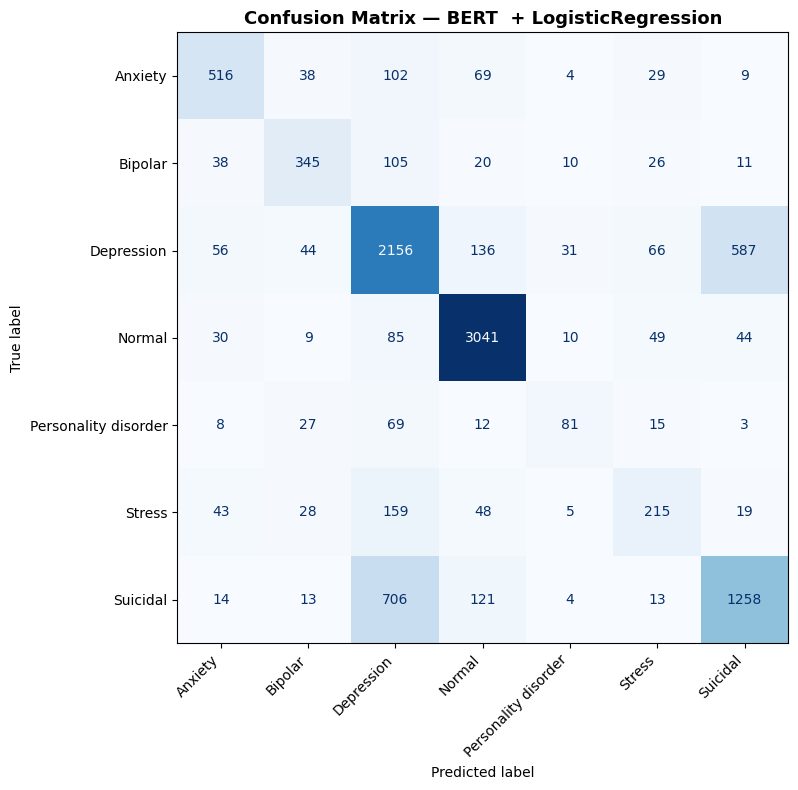
\includegraphics[width=0.75\textwidth]{matriceConfusion_BERT_LR_DIOGO.png}
  \caption{Matrice de confusion --- BERT sans fine-tuning + LR (Diogo)}
\end{figure}
\end{center}

\begin{note}[Interprétation des résultats]
Les résultats pour un BERT non fine-tuné ici sont logiques, il s'agit d'une baseline 
solide qui montre que les embeddings \texttt{[CLS]} contiennent déjà une information 
pertinente pour la classification de sentiments, \textbf{même sans adaptation spécifique à 
notre dataset.}\\
Cependant, \textbf{les performances sont généralement inférieures} à celles obtenues avec un 
fine-tuning complet (Modèle B), ce qui souligne l'importance de l'adaptation du modèle
aux particularités de la tâche.
\end{note}


\pagebreak
% ══════════════════════════════════════════════════════════════════════════════
\section{Modèle B — BERT avec fine-tuning}

\subsection{Principe du fine-tuning}

Dans cette seconde approche, \textbf{tous les poids de BERT sont mis à jour} pendant
l'entraînement, y compris les couches d'attention. On ajoute en sortie une
\textbf{tête de classification} (couche \texttt{Linear}) qui projette le vecteur
\texttt{[CLS]} vers les \texttt{num\_labels} classes.

\begin{figure}[H]
\begin{center}
\begin{tikzpicture}[
  scale=0.85,
  transform shape,
  node distance=15mm,
  >=Latex,
  box/.style={rounded corners, draw=blue!70!black, thick, fill=blue!5,
              align=center, text width=3.2cm, minimum height=1.2cm,
              inner sep=6pt, font=\small},
  arrow/.style={-Latex, thick, draw=blue!70!black},
  label/.style={font=\footnotesize, color=blue!70!black, align=center}
]

%% ── Noeuds ──────────────────────────────────────────────────────────
\node[box, text width=5cm] (text) {Texte brut\\[4pt]
  \textit{"Le chat mange la souris"}};

\node[box, right=of text, text width=7cm] (token) {Tokens\\[4pt]
  \texttt{[CLS]} \textit{Le chat mange la souris} \texttt{[SEP]}};

\node[box, below=2cm of token, xshift=2cm] (emb) {Embeddings\\[4pt]
  vecteur 768 dim\\par token};

\node[box, left=of emb] (cls) {Vecteur \texttt{[CLS]}\\[4pt]
  représentation\\globale de la phrase};

\node[box, left=of cls] (logits) {Logits\\[4pt]
  \textit{log-probabilités}\\par classe};

%% ── Noeud Loss + backprop (dessous, centré entre cls et logits) ──
\node[box, fill=red!5, draw=red!60!black,
  below=18mm of cls] (loss)
  {Loss + Backprop\\[4pt]
  \texttt{CrossEntropyLoss}\\
  $\rightarrow$ \texttt{AdamW}};

%% ── Flèches principales ─────────────────────────────────────────
\draw[arrow] (text)   -- (token);
\draw[arrow] (token.east)  -- ++(2cm,0) -| ++(0,-3.65cm) -- (emb.east);
\draw[arrow] (emb)    -- (cls);
\draw[arrow] (cls)    -- (logits);

%% ── Flèche loss ─────────────────────────────────────────────────
\draw[arrow, draw=red!60!black]
  (logits.south) |- (loss.west);
\draw[arrow, draw=red!60!black, dashed]
  (loss.east) -| node[below, font=\footnotesize, color=red!60!black]
  {mise à jour des poids} (emb.south);

%% ── Annotations sous les flèches ───────────────────────────────
\node[label] at ($(text)!0.5!(token) + (-0.5,-1)$)
  {\texttt{BertTokenizer}};

\node[label] at ($(token)!0.5!(emb) + (6,-.3)$)
  {Embedding\\layer};

\node[label] at ($(emb)!0.5!(cls) + (0,-1.6)$)
  {12$\times$ Transformer\\block};

\node[label] at ($(cls)!0.5!(logits) + (0,-1.6)$)
  {Linear(768\,$\rightarrow$\,\textit{n})\\+ Softmax};

\end{tikzpicture}
\caption{\centering\small Schéma simplifié du pipeline de fine-tuning de BERT
  pour la classification de texte (Modèle B).}
\end{center}
\end{figure}

\begin{center}
\begin{tabular}{@{}lll@{}}
  \toprule
  Critère & Modèle A (sans fine-tuning) & Modèle B (avec fine-tuning) \\
  \midrule
  Poids BERT & Gelés & Mis à jour \\
  Temps d'entraînement & Court & Long (GPU recommandé) \\
  Mémoire & Faible & Élevée \\
  Performances attendues & Baseline & Meilleures \\
  Données nécessaires & Peu & Quelques milliers suffisent \\
  \bottomrule
\end{tabular}
\end{center}

\subsection{Préparation du Dataset PyTorch}

PyTorch utilise des objets \texttt{Dataset} et \texttt{DataLoader} pour gérer l'itération
sur les données par batchs pendant l'entraînement. Une classe \texttt{MentalHealthDataset}
encapsule les tenseurs tokenisés et les labels. Le \texttt{DataLoader} est configuré avec
\texttt{batch\_size=16} (ou 32 selon la mémoire GPU) et \texttt{shuffle=True} pour le
train uniquement.

\begin{tipbox}[Pourquoi mélanger (\texttt{shuffle=True}) ?]
Mélanger les exemples à chaque epoch évite que le modèle apprenne l'ordre des données.
\textbf{Cela stabilise la convergence et réduit le risque de sur-apprentissage.}
\end{tipbox}

\subsection{Chargement du modèle et tête de classification}

\texttt{BertForSequenceClassification} est le modèle officiel Hugging Face pour la
classification de texte. Il intègre automatiquement~:
\begin{itemize}[leftmargin=1.5cm]
  \item Le \texttt{BertModel} de base (12 couches Transformer)~;
  \item Un \texttt{Dropout(0.1)}\footnote[1]{Mécanisme de régularisation qui désactive aléatoirement une fraction des neurones
pendant l'entraînement. Cela empêche le modèle de trop dépendre de certains neurones
et améliore la généralisation.} appliqué au vecteur \texttt{[CLS]}~;
  \item Une couche \texttt{Linear(768, num\_labels)} comme tête de classification.
\end{itemize}

\textbf{Optimiseur~:} \texttt{AdamW} avec un \textit{learning rate} de $2\times10^{-5}$,
valeur recommandée par l'équipe Google pour le fine-tuning BERT.

\begin{tipbox}[Pourquoi AdamW et pas Adam ?]
AdamW est utilisé à la place d'Adam classique, car il corrige la gestion du \textit{weight decay}\footnotetext{\textit{[\ldots] 'Loshchilov and Hutter 2017 discovered that L2 regularization is not effective in Adam, and proposed AdamW' [\ldots]}
(\href{https://docs.graphcore.ai/projects/bert-training/en/latest/bert.html}{Loshchilov \& Hutter, 2019})}.
Son usage pour le fine-tuning BERT s'est imposé via les scripts officiels de Hugging Face, 
les hyperparamètres recommandés étant issus de l'\href{https://mccormickml.com/2019/07/22/BERT-fine-tuning/}{Appendix A.3} du papier BERT.
\end{tipbox}

\textbf{Scheduler~:} un \texttt{get\_linear\_schedule\_with\_warmup} fait décroître le
learning rate linéairement jusqu'à 0 au fil des epochs. Cela évite des mises à jour trop
agressives en fin d'entraînement, qui pourraient déstabiliser les poids pré-entraînés.

\subsection{Boucle d'entraînement}

La boucle suit le schéma classique PyTorch, répété sur \texttt{num\_epochs} epochs
(2 à 4 suffisent généralement pour BERT)~:

\begin{lstlisting}[language={}]
Pour chaque epoch :
    model.train()
    Pour chaque batch :
        1. Envoyer le batch sur le device (GPU/CPU)
        2. Passage avant (forward) -> logits et loss
        3. Retropropagation (loss.backward())
        4. Clipper les gradients (clip_grad_norm_, max_norm=1.0)
        5. Mise a jour des poids (optimizer.step())
        6. Mise a jour du scheduler (scheduler.step())
        7. Remise a zero des gradients (optimizer.zero_grad())
    Afficher la loss moyenne de l'epoch
\end{lstlisting}

\begin{warnbox}[Gradient clipping]
L'appel \texttt{clip\_grad\_norm\_(max\_norm=1.0)} est essentiel pour BERT~: il empêche
les gradients d'exploser lors des premières epochs, ce qui peut déstabiliser les poids
pré-entraînés et faire diverger l'entraînement.
\end{warnbox}

\begin{warnbox}[Temps d'exécution]
Environ 15 à 30 minutes par epoch sur GPU (Colab T4), 2 à 3 heures sur CPU.
\textbf{L'utilisation d'un GPU est fortement recommandée.}
\end{warnbox}

\subsection{Évaluation}

Une fonction \texttt{predict(model, dataloader, device)} itère sur les batchs en mode \\
\texttt{torch.no\_grad()}, applique un \texttt{argmax} sur les logits et retourne les
tableaux \texttt{y\_true} et \texttt{y\_pred}. Les métriques sont ensuite calculées
identiquement au Modèle~A.

\subsection{Résultats obtenues — Diogo, Ulysse, Victor et Emin}

Étant la méthode la plus apprécié par l'équipe, Diogo, Ulysse, Victor et Emin se sont occupé de 
celle-ci, les résultats obtenues sont les suivants:\\

\begin{center}
\textbf{Fine Tuning} pour chaque epoch~:\\
\bigskip
\begin{tabular}{@{}C{2cm}c@{}}
  \toprule
  \textbf{Epoch} & \textbf{Loss moyenne} \\
  \midrule
  1 & 0.6361 \\
  2 & 0.3871 \\
  3 & 0.2705 \\
  \bottomrule
\end{tabular}
\end{center}

\vspace{0.5cm}

\begin{center}
\textbf{Résultat sur l'ensemble test~:}\\
\bigskip
\begin{tabular}{@{}lc@{}}
  \toprule
  \textbf{Modèle} & \textbf{Accuracy test}\\
  \midrule
  BERT \textbf{avec fine-tuning} & \textbf{0.8302} \\
  \bottomrule
\end{tabular}
\end{center}

\vspace{0.5cm}

\begin{center}
\textbf{Classification Report~:}\\
\bigskip
\begin{tabular}{@{}lccc@{}}
  \toprule
  Classe & Precision & Recall & F1-score \\
  \midrule
             Anxiety   &    0.88   &   0.89   &   0.89\\
             Bipolar   &    0.86   &   0.85   &   0.86\\
          Depression   &    0.78   &   0.77   &   0.78\\
              Normal   &    0.95   &   0.95   &   0.95\\
Personality disorder   &    0.77   &   0.68   &   0.72\\
              Stress   &    0.73   &   0.76   &   0.74\\
            Suicidal   &    0.72   &   0.73   &   0.72\\
  \bottomrule
\end{tabular}
\end{center}

\pagebreak

\begin{center}
\textbf{Matrice de confusion}~:\\
\bigskip
\begin{figure}[H]
  \centering
  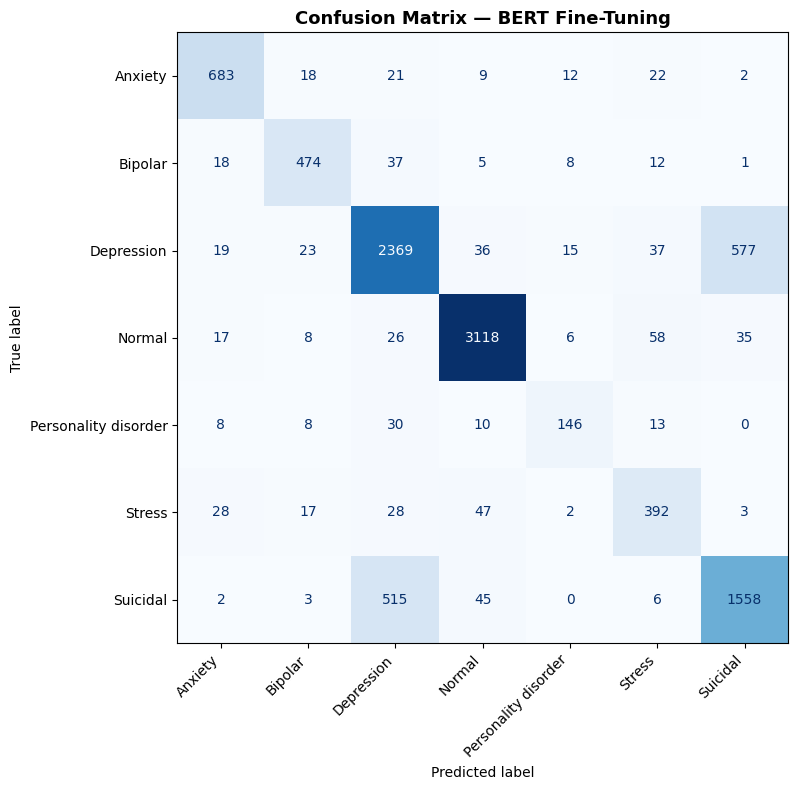
\includegraphics[width=0.75\textwidth]{matriceConfusion_BERT_FT_DIOGO.png}
  \caption{Matrice de confusion --- BERT avec fine-tuning (Diogo)}
\end{figure}
\end{center}

\begin{note}[Interprétation des résultats]
On remarque une amélioration significative de l'accuracy (0.7231 $\rightarrow$ 0.8302) grâce au fine-tuning. 
Les classes les plus difficiles à prédire (Personality disorder, Stress, Suicidal) voient une nette augmentation de leur F1-score, 
ce qui suggère que BERT a appris des représentations plus discriminantes pour ces catégories complexes.
\end{note}

\pagebreak
% ══════════════════════════════════════════════════════════════════════════════
\section{Modèle C — BERT spécialisé + fine-tuning}

\subsection{Pourquoi un modèle spécialisé?}

Le Modèle~B part de \texttt{bert-base-uncased}, pré-entraîné sur Wikipedia et
BooksCorpus — un corpus de texte très éloigné du langage émotionnel ou clinique. Le
Modèle~C part d'un BERT \textbf{déjà fine-tuné sur des tâches d'analyse de sentiments},
ce qui lui donne une meilleure représentation initiale des émotions avant même de voir
notre dataset.

\begin{center}
\begin{tabular}{@{}lll@{}}
  \toprule
  Critère & BERT-base (Modèle B) & Modèle spécialisé (Modèle C) \\
  \midrule
  Pré-entraînement initial & Wikipedia / BooksCorpus & Wikipedia / BooksCorpus \\
  Fine-tuning intermédiaire & Non & Oui — Sentiments \\
  Point de départ & Général & Spécialisé \\
  Fine-tuning sur notre data & Oui & Oui \\
  Performances attendues & Bonnes & Meilleures (théoriquement) \\
  \bottomrule
\end{tabular}
\end{center}

\subsection{Variantes de bases BERT disponibles}

Avant de présenter les modèles candidats, il convient de rappeler les principales
architectures de base utilisées dans cet écosystème~:

\subsubsection{RoBERTa (\textit{Robustly Optimized BERT Pretrained Approach})}

Amélioration de BERT proposée par Facebook en 2019. Même architecture de base, mais
avec des choix d'entraînement sensiblement améliorés~:
\begin{itemize}[leftmargin=1.5cm]
  \item \textbf{Suppression du NSP} (jugé inutile et potentiellement nuisible)~;
  \item Entraîné sur \textbf{10 fois plus de données} (160~Go contre $\sim$16~Go)~;
  \item \textbf{Dynamic masking}~: les tokens masqués changent à chaque epoch au lieu
    d'être figés~;
  \item Entraîné plus longtemps avec de plus gros batchs.
\end{itemize}
En pratique, RoBERTa surpasse BERT-base sur quasi toutes les tâches de classification
et est aujourd'hui la base la plus utilisée pour l'analyse de sentiments.

\subsubsection{DistilBERT}

Version \textbf{distillée} de BERT-base par Hugging Face (2019). Le principe~: on
entraîne un modèle compact (66~M de paramètres, 6 couches) à imiter le comportement
du grand modèle.

\begin{center}
\begin{tabular}{@{}ll@{}}
  \toprule
  Caractéristique & Valeur \\
  \midrule
  Paramètres & 66~M (vs 110~M pour BERT-base) \\
  Vitesse & $\sim$40\,\% plus rapide \\
  Taille mémoire & $\sim$40\,\% plus légère \\
  Performances & $\sim$97\,\% de BERT-base \\
  \bottomrule
\end{tabular}
\end{center}

Il est particulièrement choisi pour éviter les contraintes GPU. En revanche, sur une
tâche difficile comme la santé mentale avec 7 classes, la perte de capacité peut se
faire sentir.

\subsubsection{RoBERTa-large}

Version «~grande~» de RoBERTa~: 355~M de paramètres, 24 couches au lieu de 12.
Significativement plus performante que RoBERTa-base, mais bien plus coûteuse à
fine-tuner.

\subsection{Modèles disponibles sur Hugging Face}

Le tableau suivant recense les modèles pertinents disponibles sur Hugging Face, tous
pré-entraînés sur des données d'analyse de sentiments~:

\begin{center}
\begin{tabular}{@{}L{4.5cm}C{2cm}C{3.2cm}C{0.8cm}C{2cm}@{}}
  \toprule
  Identifiant HF & Base & Pré-entraîné sur\dots & Classes & Points forts \\
  \midrule
  \texttt{cardiffnlp/twitter-} \newline \texttt{roberta-base-sentiment} \newline \texttt{-latest} & RoBERTa & $\sim$124~M tweets & 3 & Texte informel \\
  \texttt{nlptown/bert-base-} \newline \texttt{multilingual-uncased} \newline \texttt{-sentiment} & BERT multilingual & Avis produits & 5 & Multi-langue \\
  \texttt{siebert/sentiment-} \newline \texttt{roberta-large-english} & RoBERTa-large & 15 datasets & 2 & Généralisation \\
  \texttt{j-hartmann/emotion-} \newline \texttt{english-distilroberta} \newline \texttt{-base} & DistilRoBERTa & 6 datasets émotions & 7 & Émotions fines \\
  \bottomrule
\end{tabular}
\end{center}

\begin{note}[Modèle retenu~: \texttt{j-hartmann/emotion-english-distilroberta-base}]
Le modèle retenu est \texttt{j-hartmann/emotion-english-distilroberta-base}, basé sur
DistilRoBERTa et pré-entraîné sur 6~datasets d'émotions (joie, colère, tristesse, peur,
surprise, dégoût, neutre). Ce choix est motivé par la nature du corpus~: les textes liés
à la santé mentale sont chargés émotionnellement, et ce modèle a déjà appris à
discriminer des émotions proches (tristesse vs peur, par exemple) — exactement ce qui
est requis pour distinguer Depression, Stress et Suicidal.
\end{note}

\begin{tipbox}[DistilBERT — le compromis vitesse/performance]
DistilBERT est une version allégée de BERT (66 millions de paramètres contre 110~M)~:
40\,\% plus rapide, 60\,\% plus léger, avec environ 97\,\% des performances de
BERT-base. Il est particulièrement adapté lorsque les ressources GPU sont limitées.
Compter environ \textbf{25~minutes} pour 3~epochs d'entraînement.
\end{tipbox}

\subsection{Adaptation de la tête de classification}

Le modèle importé a été fine-tuné pour un certain nombre de classes (souvent 2 ou 3
pour positif/négatif/neutre, dans notre cas 6). Notre dataset possède 7 classes. Il faut donc
\textbf{remplacer la tête de classification} par une nouvelle couche adaptée.

\begin{lstlisting}[language=Python]
model = AutoModelForSequenceClassification.from_pretrained(
    model_name,
    num_labels=num_labels,
    ignore_mismatched_sizes=True   # tete remplacee
)
\end{lstlisting}

Le paramètre \texttt{ignore\_mismatched\_sizes=True} est indispensable~: la tête
originale est remplacée par une nouvelle tête à \texttt{num\_labels}
classes — les dimensions ne correspondent plus, sans ce paramètre PyTorch lèverait
une erreur.

\subsection{Fine-tuning et évaluation}

La boucle d'entraînement est identique à celle du Modèle~B. Seul le modèle chargé
change. Le tokeniseur doit également être celui du Modèle~C — chaque modèle Hugging
Face possède son propre tokeniseur, chargé via \texttt{AutoTokenizer} pour garantir la
compatibilité.


\begin{figure}[H]
\begin{center}
\begin{tikzpicture}[
  scale=0.75,
  transform shape,
  node distance=8mm,
  >=Latex,
  box/.style={rounded corners, draw=blue!70!black, thick, fill=blue!5,
              align=center, text width=3.2cm, minimum height=1.2cm,
              inner sep=6pt, font=\small},
  boxhf/.style={box, fill=green!8, draw=green!60!black},
  boxnew/.style={box, fill=orange!8, draw=orange!60!black},
  arrow/.style={-Latex, thick, draw=blue!70!black},
  arrowred/.style={-Latex, thick, draw=red!60!black},
  label/.style={font=\footnotesize, color=blue!70!black, align=center},
  group/.style={draw=green!60!black, rounded corners, dashed, inner sep=12pt, thick},
]

%% ── Phase 0 : Texte brut ────────────────────────────────────────────────
\node[box] (text) {Texte brut\\[4pt]
  \textit{"Le chat mange la souris"}};

%% ── Phase 1 : AutoTokenizer ─────────────────────────────────────────────
\node[box, right=3cm of text] (token) {Tokens\\[4pt]
  \texttt{[CLS]} \textit{Le chat}\\
  \textit{mange\dots} \texttt{[SEP]}};

%% ── Phase 4 : Vecteur [CLS] ─────────────────────────────────────────────
\node[boxhf, below=2cm of text] (cls) {Vecteur \texttt{[CLS]}\\[4pt]
  représentation\\globale (768~dim)};

%% ── Phase 3 : Encodeur DistilRoBERTa (6 couches) ────────────────────────
\node[boxhf, right=2cm of cls] (enc) {6$\times$ Transformer\\[4pt]
  poids pré-entraînés\\mis à jour};

%% ── Phase 2 : Embeddings DistilRoBERTa ──────────────────────────────────
\node[boxhf, right=3.2cm of enc] (emb) {Embeddings\\[4pt]
  vecteur 768~dim\\par token};

%% ── Phase 5 : Nouvelle tête (remplacée) ─────────────────────────────────
\node[boxnew, below=18mm of cls] (head) {Nouvelle tête\\[4pt]
  \texttt{Linear(768\,$\to$\,7)}\\
  \texttt{+ Softmax}};

%% ── Phase 6 : Loss + Backprop ───────────────────────────────────────────
\node[box, fill=red!5, draw=red!60!black,
      right=14mm of head] (loss)
  {Loss + Backprop\\[4pt]
  \texttt{CrossEntropyLoss}\\
  $\rightarrow$ \texttt{AdamW}};

%% ── Phase 7 : Sortie ────────────────────────────────────────────────────
\node[box, right=14mm of loss] (out) {Classe prédite\\[4pt]
  ex.\ \textit{Suicidal}\\
  \textit{Depression\dots}};

%% ── Flèches principales (rangée du haut) ────────────────────────────────
\draw[arrow] (text)  -- (token);
\draw[arrow] (token.east) -- ++(0,0) -| (emb.north);
\draw[arrow] (emb)   -- (enc);
\draw[arrow] (enc)   -- (cls);

%% ── Descente vers la tête ───────────────────────────────────────────────
\draw[arrow] (cls.south) -- (head.north);

%% ── Rangée du bas ───────────────────────────────────────────────────────
\draw[arrow] (head) -- (loss);
\draw[arrow] (loss) -- (out);

%% ── Flèche backprop (pointillée, remonte vers encodeur) ─────────────────
\draw[arrowred, dashed]
  (loss.north) -- ++(0,0.6)
  -| node[near start, above, font=\footnotesize, color=red!60!black]
     {mise à jour des poids} (enc.south);

%% ── Annotations sous les flèches (rangée du haut) ──────────────────────
\node[label] at ($(text)!0.5!(token)+(0,0)$)
  {\texttt{AutoTokenizer}\\[4pt]\texttt{max\_length=128}};

\node[label] at ($(token)!0.5!(emb)+(1,1.9)$)
  {Embedding\\[4pt]layer};

\node[label] at ($(emb)!0.5!(enc)+(0,-0.2)$)
  {DistilRoBERTa\\[4pt](pré-entraîné\\émotions)};

\node[label] at ($(enc)!0.5!(cls)+(0,0)$)
  {Encodage\\[4pt]contextuel};

%% ── Annotation remplacement tête ────────────────────────────────────────
\node[font=\footnotesize, color=orange!70!black, align=center,
      below=4pt of head] (headlabel)
  {\texttt{ignore\_mismatched\_sizes=True}\\
   tête originale (2--3 classes)\\remplacée par 7 classes};

%% ── Badge modèle source (Hugging Face) ──────────────────────────────────
\node[draw=green!60!black, fill=green!8, rounded corners,
      font=\footnotesize, align=center, inner sep=5pt,
      above=6pt of enc] (badge)
  {\textbf{j-hartmann/emotion-english-distilroberta-base}\\
   pré-entraîné sur 6 datasets d'émotions (7 classes~: joie, colère\dots)};

\end{tikzpicture}
\caption{\centering\small Schéma du pipeline du Modèle~C~: DistilRoBERTa pré-entraîné
  sur des émotions (\texttt{j-hartmann/emotion-english-distilroberta-base}), tête de
  classification remplacée (\texttt{ignore\_mismatched\_sizes=True}) et fine-tuné sur
  7 classes de santé mentale.}
\end{center}
\end{figure}

\subsection{Résultats obtenues — Logan}

Contrairement à celle précédente, celle-ci est un peu plus complexe et donc a été réalisée par Logan seul, les résultats obtenues sont les suivants:\\


\begin{center}
\textbf{Fine Tuning} pour chaque epoch~:\\
\bigskip
\begin{tabular}{@{}C{2cm}c@{}}
  \toprule
  \textbf{Epoch} & \textbf{Loss moyenne} \\
  \midrule
  1 & 0.6483 \\
  2 & 0.4305 \\
  3 & 0.3156 \\
  \bottomrule
\end{tabular}
\end{center}

\vspace{1cm}

\begin{center}
\textbf{Résultat sur l’ensemble test}:\\
\bigskip
\begin{tabular}{@{}lc@{}}
  \toprule
  \textbf{Modèle} & \textbf{Accuracy test}\\
  \midrule
  BERT \textbf{spécialisé avec fine-tuning} & \textbf{0.8343} \\
  \bottomrule
\end{tabular}
\end{center}

\vspace{1cm}

\begin{center}
\textbf{Classification Report}~:\\
\bigskip
\begin{tabular}{@{}lccc@{}}
  \toprule
  Classe & Precision & Recall & F1-score \\
  \midrule
             Anxiety   &    0.87   &   0.90   &   0.88\\
             Bipolar   &    0.87   &   0.83   &   0.85\\
          Depression   &    0.80   &   0.76   &   0.78\\
              Normal   &    0.96   &   0.95   &   0.96\\
Personality disorder   &    0.69   &   0.73   &   0.71\\
              Stress   &    0.74   &   0.78   &   0.76\\
            Suicidal   &    0.71   &   0.76   &   0.73\\
  \bottomrule
\end{tabular}
\end{center}

\pagebreak

\begin{center}
\textbf{Matrice de confusion}~:\\
\bigskip
\begin{figure}[H]
  \centering
  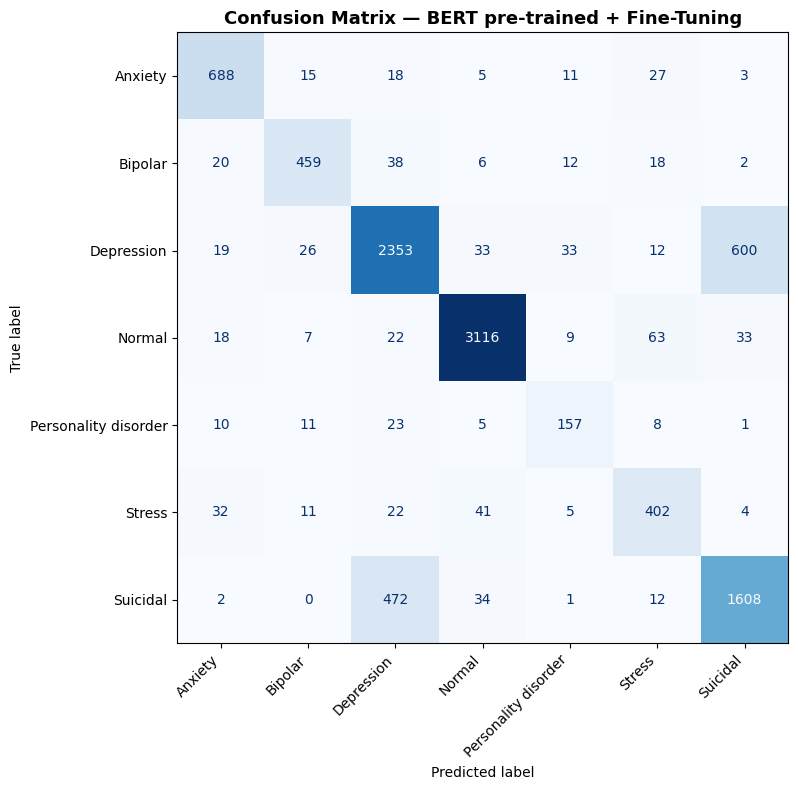
\includegraphics[width=0.75\textwidth]{matriceConfusion_BERT_PT_FT_LOGAN.png}
  \caption{Matrice de confusion --- BERT pré-entrainé avec fine-tuning (Logan)}
\end{figure}
\end{center}

\begin{note}[Interprétation des résultats]
Le Modèle~C, avec une accuracy de \textbf{0.8343}, surpasse légèrement le Modèle~B (0.8302).
L'amélioration est particulièrement notable sur les classes difficiles (Personality disorder, Stress, Suicidal), 
suggérant que le pré-entraînement sur des émotions a permis au modèle de mieux capturer les nuances émotionnelles 
présentes dans ces catégories. Cependant, \textbf{les gains restent modestes}, ce qui indique que le fine-tuning sur notre dataset 
a déjà permis au Modèle~B d'apprendre des représentations efficaces.
\end{note}

\pagebreak
% ══════════════════════════════════════════════════════════════════════════════
\section{Comparaison globale des modèles}

\subsection{Tableau récapitulatif}

Le tableau ci-dessous synthétise les performances des cinq modèles (Naive Bayes
et K-Means issus du notebook principal, plus les trois variantes BERT). Les valeurs
marquées d'un point d'interrogation seront renseignées à l'issue de l'implémentation.

\begin{center}
\begin{tabular}{@{}L{4cm}C{2.5cm}C{3cm}L{3.5cm}@{}}
  \toprule
  Modèle & Accuracy test & Temps approx. & Remarque \\
  \midrule
  K-Means + W2V & 0.20 & Quelques minutes & Non supervisé \\
  K-Means + TF-IDF & 0.4636 & Quelques minutes & Non supervisé \\
  Naive Bayes + BoW & 0.6666 & Quelques secondes & Supervisé \\
  Naive Bayes + TF-IDF & 0.6927 & Quelques secondes & Supervisé \\
  LinearSVC + BoW & 0.7309 & Quelques minutes & Supervisé \\
  Logistic Regression + TF-IDF & 0.7532 & Quelques secondes & supervisé \\
  LinearSVC + TF-IDF & 0.7586 & Quelques minutes & Supervisé \\
  \midrule
  BERT sans fine-tuning (A) & 0,7231 & Minutes (CPU) & Baseline BERT \\
  BERT avec fine-tuning (B) & 0,8302 & Heures (GPU) & Fine-tuning complet \\
  BERT spécialisé + FT (C) & 0.8343 & ~30min (GPU) \newline 2-3h (CPU) & Meilleur point de départ \\
  \bottomrule
\end{tabular}
\end{center}


\subsection{Que peut-on en conclure?}

\subsubsection{1. Quel modèle obtient la meilleure accuracy~?}
On remarque que globalement les modèles \textbf{BERT surpassent largement les méthodes classiques}, 
avec un gain d'environ 8 points de pourcentage. Cela illustre la puissance des représentations 
contextuelles et du pré-entraînement massif de BERT .

\subsubsection{2. Apport du fine-tuning (Modèle B vs Modèle A)}
L'apport du fine tuning est clairement visible (Modèle B vs A), avec une amélioration de plus de 10 points d'accuracy.
Le Modèle C, malgré son pré-entraînement spécialisé, n'apporte qu'une amélioration marginale par rapport au Modèle B, 
suggérant que le fine-tuning sur notre dataset a déjà permis d'extraire des représentations efficaces, 
et que le gain du pré-entraînement spécialisé est limité dans ce cas.

\subsubsection{3. Modèle spécialisé vs BERT-base (Modèle C vs Modèle B)}
Le compromis coût/performance penche en faveur du Modèle B pour une utilisation en production,
car il offre une excellente performance pour un coût d'entraînement raisonnable, tandis que le Modèle C, bien que légèrement meilleur,
nécessite un pré-entraînement plus coûteux et n'apporte qu'un gain marginal.
Malgrès une grande amélioration des classes difficiles (Personality disorder, Stress, Suicidal) avec les modèles BERT,
ces classes restent les plus problématiques. 

\subsubsection{4. Classes difficiles}
On remarque que \textit{Depression} et \textit{Suicidal} restent souvent confondus, 
ce qui suggère que même les modèles les plus avancés ont du mal à capturer les nuances entre ces catégories émotionnellement proches.


\subsection{Points de vigilance}

\begin{itemize}[leftmargin=1.5cm]
  \item \textbf{Limite de 512 tokens~:} dans notre dataset, la majorité des textes
    dépassent rarement 128 tokens après nettoyage, ce qui limite l'impact de la
    troncature. La valeur \texttt{max\_length=128} est donc un bon compromis.
  \item \textbf{Déséquilibre des classes~:} comme dans le notebook principal, Depression
    est sur-représentée. Les métriques macro (F1 macro) doivent être privilégiées pour
    ne pas masquer les mauvaises performances sur les classes minoritaires.
  \item \textbf{Confusion Depression/Suicidal~:} ce problème persistant dans toutes les
    méthodes classiques pointait vers une limite des données. BERT, grâce à ses
    représentations contextuelles, pourrait partiellement atténuer cette confusion — à
    vérifier expérimentalement.
  \item \textbf{Reproductibilité~:} les seeds sont fixées à 42 pour \texttt{random},
    \texttt{numpy} et \texttt{torch} afin de garantir la reproductibilité des
    résultats entre exécutions.
\end{itemize}

\pagebreak
% ══════════════════════════════════════════════════════════════════════════════
\section*{Références}
\addcontentsline{toc}{section}{Références}

\textbf{Papier de référence}
\begin{itemize}[leftmargin=1.5cm]
  \item Devlin, J., Chang, M.-W., Lee, K., \& Toutanova, K. (2018).
    \textit{BERT: Pre-training of Deep Bidirectional Transformers for Language
    Understanding}. \url{https://arxiv.org/pdf/1810.04805}
  \item Wolf, T. et al. (2020). \textit{Transformers: State-of-the-Art Natural Language
    Processing}. \url{https://arxiv.org/pdf/1910.03771}
  \item Loshchilov \& Hutter (2019)
    \textit{Pre-Training and Fine-Tuning BERT for the IPU}
    \url{https://docs.graphcore.ai/projects/bert-training/en/latest/bert.html}
\end{itemize}

\textbf{Modèles Hugging Face}
\begin{itemize}[leftmargin=1.5cm]
  \item RoBERTa — Hugging Face. 
    \url{https://huggingface.co/docs/transformers/model_doc/roberta}
  
  \item RoBERTa-large — Hugging Face. 
    \url{https://huggingface.co/docs/transformers/model_doc/roberta_large}

  \item DistilBERT — Hugging Face. 
    \url{https://huggingface.co/docs/transformers/model_doc/distilbert}

  \item cardiffnlp/twitter-roberta-base-sentiment-latest — Hugging Face.
    \url{https://huggingface.co/cardiffnlp/twitter-roberta-base-sentiment-latest}

  \item nlptown/bert-base-multilingual-uncased-sentiment — Hugging Face.
    \url{https://huggingface.co/nlptown/bert-base-multilingual-uncased-sentiment}

  \item siebert/sentiment-roberta-large-english — Hugging Face.
    \url{https://huggingface.co/siebert/sentiment-roberta-large-english}

  \item j-hartmann/emotion-english-distilroberta-base — Hugging Face.
    \url{https://huggingface.co/j-hartmann/emotion-english-distilroberta-base}
\end{itemize}

\textbf{Ressources}
\begin{itemize}[leftmargin=1.5cm]
    \item Sentiment Analysis for Mental Health — Kaggle.
    \url{https://www.kaggle.com/datasets/suchintikasarkar/sentiment-analysis-for-mental-health}
\end{itemize}

\end{document}